\section{Power}
\label{sec:power}

\subsection{\SI{12}{\volt} Input Protection}

As \SI{12}{\volt} input protection we use a TPS259480AYWPR Texas Instruments eFuse that features:

To safeguard the \SI{12}{\volt} supply, we employ a Texas Instruments TPS259480A e-Fuse, which integrates back-to-back MOSFETs and offers the following features:

\begin{itemize}
    \item Integrated back-to-back FETs with low ON resistance $R_\mathrm{ON}=\SI{12.2}{\milli\ohm}$.
    \item Ideal diode operation with true reverse current blocking.
    \item Fast overload protection.
    \item Overcurrent protection with load current monitor.
    \item Fast-trip response for short circuit protection.
    \item Adjustable output slew rate.
\end{itemize}

Upstream of the e-Fuse, a TI TVS1800DRV \SI{18}{\volt} flat-clamp transient-voltage suppressor absorbs voltage spikes and surges on the \SI{12}{\volt} line. Downstream, a B520C \SI{20}{\volt}, \SI{5}{\ampere} Schottky diode provides secondary overvoltage protection at the e-Fuse output. \autoref{fig:power_12vin} illustrate the complete \SI{12}{\volt} input protection circuit.

\begin{figure}[ht]
  \centering
  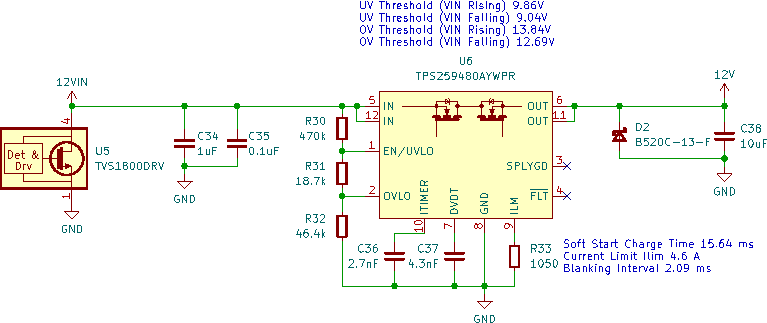
\includegraphics[width=0.8\linewidth]{sections/power/fig_12vin.pdf}
  \caption{\SI{12}{\volt} Input Protection Circuit}
  \label{fig:power_12vin}
\end{figure}


\subsection{Digital \SI{3.3}{\volt} (3V3D)}

Digital \SI{3.3}{\volt} serves as the primary supply for the Zynq SoC and feeds the \SI{2.5}{\volt} digital LDO used by the ADC. We selected the Analog Devices LT8642S synchronous step-down converter, which provides:
\begin{itemize}
    \item Ultra low EMI emissions (Silent Switcher 2 Architecture).
    \item High efficiency: up to 95\% efficiency at \SI{2}{\mega\hertz}, \SI{12}{\volt} input and \SI{3.3}{\volt} output.
    \item Up to \SI{10}{\ampere} output current.
    \item External compensation.
\end{itemize}

The LT8642S is configured to operate at \SI{2}{\mega\hertz} (see \autoref{fig:power_3v3d}). A Coilcraft XGL1010-801 shielded inductor (\SI{0.8}{\micro\henry}, \SI{0.88}{\milli\ohm} DCR) minimizes losses. Upstream of the converter input, a $\pi$ LC filter suppresses input noise. Power-Good output (\texttt{3V3D\_PG}) and the SYNC pin (\texttt{3V3D\_SYNC}) are both tied back to the Zynq SoC for voltage monitoring and clock synchronization. See LTSpice and LTPoweCAD simulation files for transient and frequency compensation design.

\begin{figure}[ht]
  \centering
  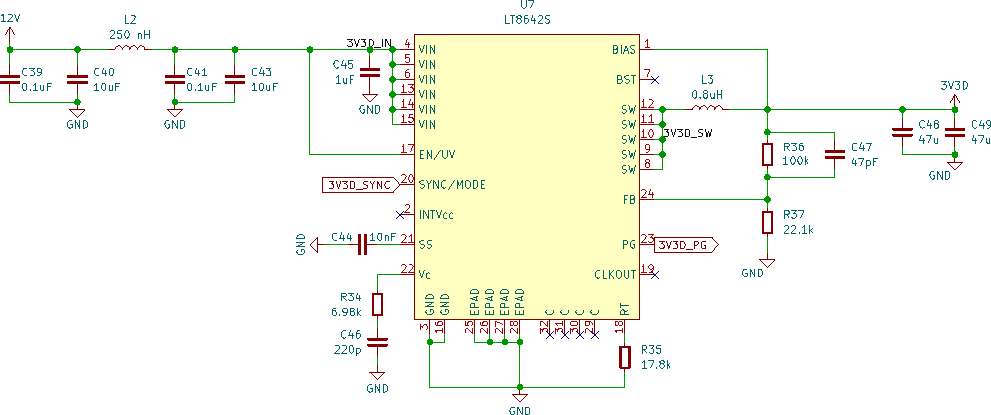
\includegraphics[width=0.8\linewidth]{sections/power/fig_3v3d.pdf}
  \caption{Digital \SI{3.3}{\volt} Step-Down DC-DC Converter Circuit}
  \label{fig:power_3v3d}
\end{figure}



\subsection{Analog \SI{5.5}{\volt} (5V5A)}

Analog \SI{5.5}{\volt} (5V5A) powers low noise analog LDO that supply analog front end and ADC. We selected the Analog Devices LT8624S synchronous step-down DC-DC converter that features:
\begin{itemize}
    \item Ultralow \SI{4}{\nano\volt/\sqrtunit{\hertz}} RMS noise (Silent Switcher 3 architecture).
    \item High efficiency.
    \item Ultra fast transient response: \SI{1}{\micro\second}.
    \item Up to \SI{4}{\ampere} continuous output current.
    \item External compensation.
\end{itemize}

The LT8624S is configured to operate at \SI{2}{\mega\hertz} (see \autoref{fig:power_5v5a}). A Coilcraft XGL1313-222 shielded inductor (\SI{2.2}{\micro\henry}, \SI{1.4}{\milli\ohm} DCR) minimizes losses. Upstream of the converter input, a $\pi$ LC filter suppresses input noise. Enable (\texttt{5V5A\_EN}), Power-Good output (\texttt{5V5A\_PG}) and the SYNC pin (\texttt{5V5A\_SYNC}) are connected to the Zynq SoC for enabling, voltage monitoring and clock synchronization. See LTSpice and LTPoweCAD simulation files for transient and frequency compensation design.

\begin{figure}[ht]
  \centering
  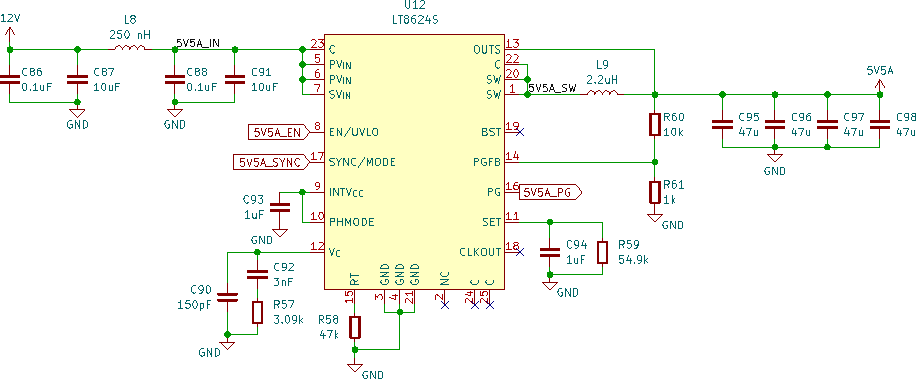
\includegraphics[width=0.8\linewidth]{sections/power/fig_5v5a.pdf}
  \caption{Analog \SI{5.5}{\volt} Step-Down DC-DC Converter Circuit}
  \label{fig:power_5v5a}
\end{figure}

\subsection{Analog \SI{15.5}{\volt} (+15V5A)}

The Analog \SI{15.5}{\volt} (+15V5A) DC-DC converter powers the low-noise Analog \SI{15}{\volt} LDO (15VA). We chose the Analog Devices LT8350S synchronous buck-boost converter that features:

\begin{itemize}
    \item 4-switch single inductor architecture.
    \item Low EMI (Silent Switcher 2 architecture).
    \item Up to 95\% efficiency at \SI{2}{\mega\hertz}.
    \item $\pm$1.5\% output voltage regulation.
    \item External compensation.
\end{itemize}

The LT8350S is configured to operate at \SI{2}{\mega\hertz} (see \autoref{fig:power_15v5a}). A Coilcraft XGL1313-222 shielded inductor (\SI{2.2}{\micro\henry}, \SI{1.4}{\milli\ohm} DCR) minimizes losses. Upstream of the converter input, a $\pi$ LC filter suppresses input noise. Enable (\texttt{15V5A\_EN}), Power-Good output (\texttt{15V5A\_PG}) and the SYNC pin (\texttt{15V5A\_SYNC}) are connected to the Zynq SoC for enabling, voltage monitoring and clock synchronization. See LTSpice and LTPoweCAD simulation files for transient and frequency compensation design.

\begin{figure}[ht]
  \centering
  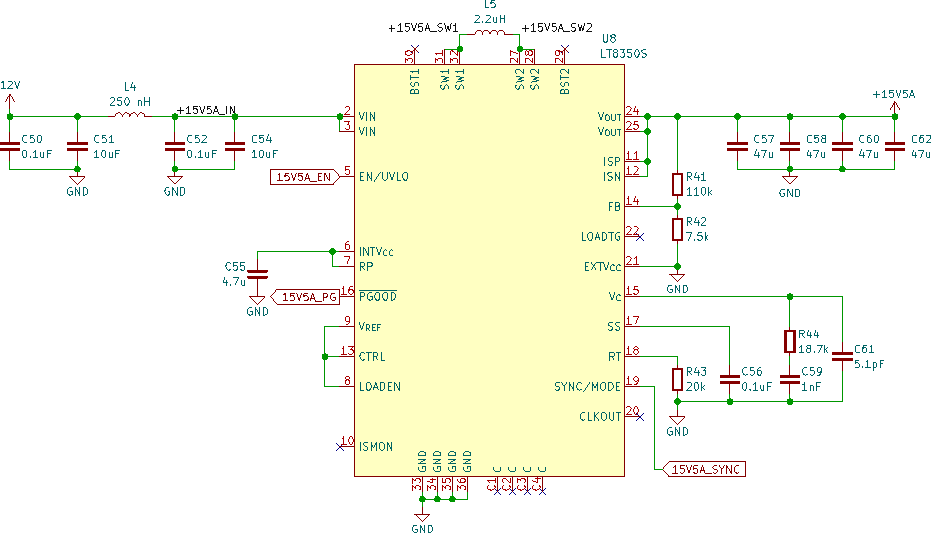
\includegraphics[width=0.8\linewidth]{sections/power/fig_15v5a.pdf}
  \caption{Analog \SI{15.5}{\volt} Buck-Boost DC-DC Converter Circuit}
  \label{fig:power_15v5a}
\end{figure}

\subsection{Analog \SI{-15.5}{\volt} (-15V5A)}

Analog \SI{-15.5}{\volt} (-15V5A) DC-DC converter powers the low-noise \SI{-15}{\volt} LDO (-15VA). We choose the Analog Devices LT3579 synchronous boost-inverting DC-DC converter that features:
\begin{itemize}
    \item \SI{6}{\ampere}, \SI{42}{\volt} combined power switch.
    \item Output short circuit protection.
    \item Configurable as inverting converter.
    \item External compensation.
\end{itemize}

The LT3579 is configured to operate at \SI{2}{\mega\hertz} (see \autoref{fig:power_n15v5a}). An Eaton DRQ-125-3R3-R coupled inductor (\SI{3.3}{\micro\henry}, \SI{6.3}{\milli\ohm} DCR) minimizes losses. Upstream of the converter input, a $\pi$ LC filter suppresses input noise. Enable (\texttt{-15V5A\_EN}), Power-Good output (\texttt{-15V5A\_PG}) and the SYNC pin (\texttt{-15V5A\_SYNC}) are connected to the Zynq SoC for enabling, voltage monitoring and clock synchronization. See LTSpice for transient design.

\begin{figure}[ht]
  \centering
  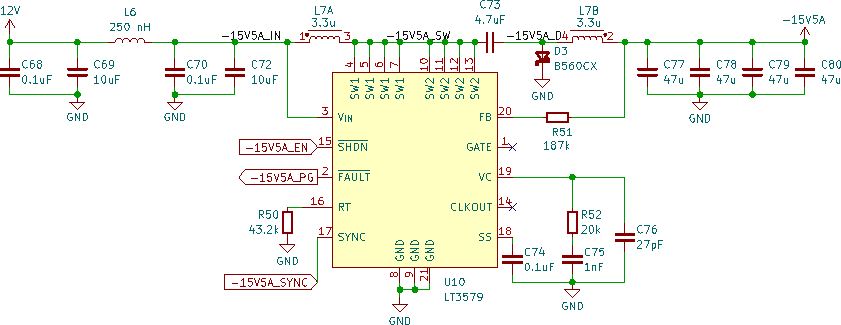
\includegraphics[width=0.8\linewidth]{sections/power/fig_n15v5a.pdf}
  \caption{Analog \SI{-15.5}{\volt} Inverting DC-DC Converter Circuit}
  \label{fig:power_n15v5a}
\end{figure}

\subsection{Linear Regulators}

The board requires multiple low-noise linear regulators to generate the analog and digital rails from the protected input supply. The following voltages are provided:
\begin{itemize}
    \item Analog Supplies: \SI{15}{\volt} (15VA), \SI{-15}{\volt} (-15VA), \SI{5}{\volt} (5VA), \SI{4.2}{\volt} (4V2A) and \SI{2.5}{\volt} (2V5A) for the analog front-end, ADCs and any external circuitry.
    \item Digital Supplies: \SI{2.5}{\volt} (2V5D) for the ADC LVDS and the Zynq SoC LVDS I/O bank.
\end{itemize}

All rails are generated by Analog Devices LT3042 (15VA), LT3093 (-15VA) and LT3045 (5VA, 4V2A, 2V5A and 2V5D ) ultra-low noise LDOs. These regulators offers:
\begin{itemize}
    \item Extremely low output noise: \SI{0.8}{\micro\volt} RMS (\SI{10}{\hertz} to \SI{100}{\kilo\hertz}) and \SI{2}{\nano\volt/\sqrtunit{\hertz}} at \SI{10}{\kilo\hertz}.
    \item Ultrahigh PSRR: \SI{73}{\decibel} (LT3093), \SI{76}{\decibel} (LT3045) and \SI{79}{\decibel} (LT3042)  at \SI{1}{\mega\hertz}.
    \item \SI{500}{\milli\ampere} (LT3045) and \SI{200}{\milli\ampere} (LT3093 and LT3042) output current.
\end{itemize}

\autoref{fig:power_5va} shows the schematic of the analog \SI{5}{\volt} regulator. Aside from the different resistor values used for setting the output voltage and the power-good feedback network, all LDO circuits follow the same layout. Each device's Enable (\texttt{EN}) and Power-Good (\texttt{PG}) pins are connected back to the Zynq SoC for centralized sequencing and fault monitoring.

\begin{figure}[ht]
  \centering
  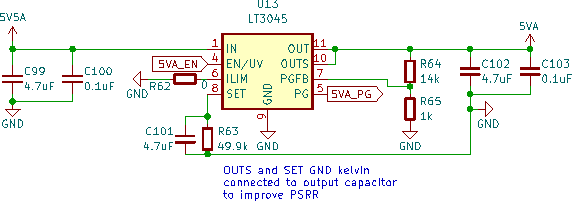
\includegraphics[width=0.8\linewidth]{sections/power/fig_5va.pdf}
  \caption{Analog \SI{5}{\volt} LDO Circuit}
  \label{fig:power_5va}
\end{figure}